\documentclass[a4paper,10pt]{article}
\usepackage{graphicx}
\usepackage[left=1in,right=1in,top=1in,bottom=1in]{geometry}
\usepackage{hyperref}
\usepackage{fancyhdr}
\usepackage{enumitem}

\pagestyle{fancy}
\lhead{\textbf{Daniel Velarde Kubber}}
\rhead{\textbf{Currículum Vitae}}
\cfoot{\thepage}

\begin{document}

% Encabezado con foto
\begin{minipage}[t]{0.7\textwidth}
\begin{center}
    {\LARGE \textbf{Daniel Velarde Kubber}}\\
    \vspace{5pt}
    \normalsize
    La Paz, Bolivia | +591 76778873 | \href{mailto:daniel.velarde.kubber@gmail.com}{daniel.velarde.kubber@gmail.com} \\
    \url{https://github.com/DanielVelarde} | \url{https://linkedin.com/in/daniel-velarde-kubber-027a8951/}
\end{center}
\end{minipage}
\hfill
\begin{minipage}[t]{0.25\textwidth}
    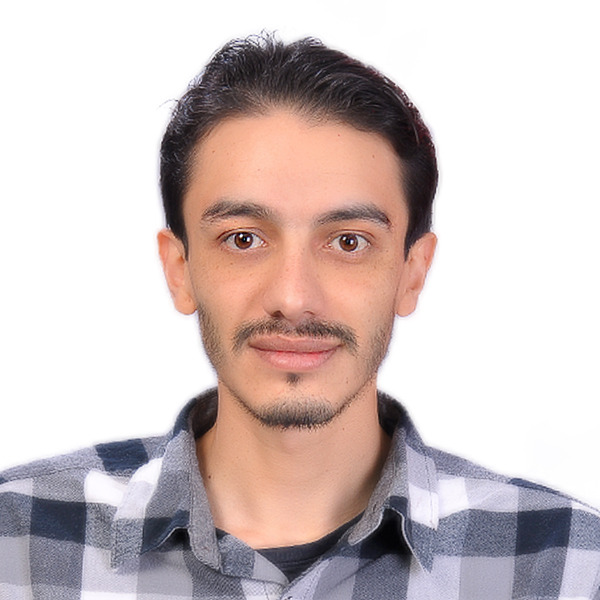
\includegraphics[width=2.5cm]{photocv.jpeg}
\end{minipage}

\vspace{10pt}

\section*{Resumen Profesional}
Ingeniero en Sistemas con sólida experiencia en bases de datos, análisis de datos, desarrollo backend con Python y SQL, creación de herramientas predictivas para mercados financieros, y tecnología Blockchain. Apasionado por el desarrollo de software, machine learning y automatización, con proyectos propios implementados y publicados en GitHub.

\vspace{10pt}

\section*{Educación}
\textbf{Ingeniería Industrial y de Sistemas} \\
Universidad Privada Boliviana — Cochabamba, Bolivia \hfill \textit{2007 - 2012}

\vspace{10pt}

\section*{Experiencia Profesional}

\textbf{Desarrollador de Herramientas Predictivas - Proyecto Independiente} \hfill \textit{Sept 2023 – Actualidad} \\
\begin{itemize}[leftmargin=*]
    \item Diseño y desarrollo de herramienta de análisis técnico predictivo usando Python, pandas, NumPy, machine learning, y visualización con Bokeh y Matplotlib.
    \item Integración con datos históricos de criptomonedas desde Binance.
    \item Arquitectura de datos organizada por pares de trading en PostgreSQL.
    \item Código fuente disponible en: \url{https://github.com/DanielVelarde/briefcase.git}
\end{itemize}

\vspace{5pt}


\textbf{Capacitador Independiente en Criptoactivos y Seguridad} \hfill \textit{Abril 2024} \\
\begin{itemize}[leftmargin=*]
    \item Dicté una capacitación a Representaciones Arequipa SRL sobre criptoactivos, enfocada en la seguridad a la hora de resguardo de valor.
\end{itemize}

\vspace{5pt}

\textbf{Docente - Universidad Católica Boliviana (Post proceso de impresión 3D)} \hfill \textit{Sept 2023 – Oct 2023} \\
\begin{itemize}[leftmargin=*]
    \item Capacitación en técnicas profesionales para post proceso de impresión 3D, incluyendo suavizado, imprimación, técnicas de aerografía y pincel.
\end{itemize}

\vspace{5pt}

\textbf{Propietario y CEO - Hobbie 3D Print} \hfill \textit{2018 – 2023} \\
\begin{itemize}[leftmargin=*]
    \item Liderazgo estratégico de la empresa, optimización de impresión 3D y desarrollo de productos con alta calidad.
\end{itemize}

\vspace{5pt}

\textbf{Especialista en Tecnología Blockchain y Programación Solidity (en aprendizaje)} \hfill \textit{2019 – Actualidad} \\
\begin{itemize}[leftmargin=*]
    \item Experiencia en tecnología Blockchain, manejo de criptomonedas y seguridad.
    \item Actualmente aprendiendo programación en Solidity para desarrollo de smart contracts.
\end{itemize}

\vspace{5pt}

\textbf{Gestor de Proyectos y DBA — Velarde Construcciones SRL} \hfill \textit{2013 – 2018} \\
\begin{itemize}[leftmargin=*]
    \item Gestión y mantenimiento de bases de datos MySQL.
    \item Desarrollo de scripts de respaldo y control de inventarios con reportes automatizados.
    \item Coordinación de tareas TI y digitalización de procesos administrativos.
\end{itemize}

\vspace{5pt}

\textbf{Administrador de Bases de Datos — Representaciones Arequipa SRL} \hfill \textit{2012 – 2013} \\
\begin{itemize}[leftmargin=*]
    \item Administración y mantenimiento de base de datos MySQL.
    \item Implementación de políticas de respaldo, seguridad de datos y despliegue en máquinas virtuales.
    \item Soporte técnico a usuarios internos y resolución de incidencias.
\end{itemize}

\vspace{10pt}

\section*{Certificaciones y Cursos}

\textbf{IBM Data Engineering Professional Certificate — Coursera} \hfill \textit{Oct 2023} \\
Certificación profesional otorgada por IBM tras completar un programa integral de 13 cursos enfocados en ingeniería de datos. \\
\url{https://www.coursera.org/account/accomplishments/specialization/W8KEPFZX9XGF}

\vspace{2pt}

\textit{Cursos completados:}
\begin{itemize}
  \item Introduction to Data Engineering
  \item Python for Data Science, AI & Development
  \item Python Project for Data Engineering
  \item Introduction to Relational Databases (RDBMS)
  \item Databases and SQL for Data Science with Python
  \item Hands-on Introduction to Linux Commands and Shell Scripting
  \item Relational Database Administration (DBA)
  \item ETL and Data Pipelines with Shell, Airflow and Kafka
  \item Data Warehouse Fundamentals
  \item Introduction to NoSQL Databases
  \item Introduction to Big Data with Spark and Hadoop
  \item Machine Learning with Apache Spark
  \item Data Engineering Capstone Project
\end{itemize}

\vspace{6pt}

\textbf{English Proficiency Certificate — Duolingo English Test} \hfill \textit{Ene 2024} \\
\textit{Overall Score: 125/160 (CEFR C1)} — Verificación oficial: \\
\url{https://certs.duolingo.com/m6cxpufhsvzed86x}

\vspace{3pt}

\textbf{TOEFL Test — Educational Testing Service} \hfill \textit{2008 (caducado)} \\
Examen académico de inglés rendido en 2008 como referencia de formación previa en el idioma.

\vspace{10pt}

\section*{Habilidades Técnicas}
\textbf{Bases de Datos:} PostgreSQL, MySQL, IBM Db2, RDBMS, NoSQL \\
\textbf{Lenguajes de Programación:} Python, SQL, C++, C\#, Bash, Solidity (aprendizaje) \\
\textbf{Herramientas de Datos:} Pandas, NumPy, Matplotlib, Bokeh, Jupyter Notebook \\
\textbf{ETL y Pipelines:} ETL, IBM Cloud, Arquitectura de Datos, Canalización de Datos \\
\textbf{DevOps y Entorno:} Linux, Git, GitHub, Docker (nivel básico), Virtualización \\
\textbf{Cripto y Blockchain:} TradingView, Binance API, Seguridad en Criptoactivos, Análisis Técnico, Smart Contracts \\
\textbf{Otros:} Visualización de Datos, Microsoft Office, IBM Watson, Desarrollo Backend

\vspace{10pt}

\section*{Proyectos Destacados}
\textbf{Herramienta Predictiva de Criptomonedas — Python + PostgreSQL + ML} \\
Desarrollo de aplicación de análisis predictivo para mercados cripto usando machine learning, ETL personalizado y arquitectura multi-par con datos históricos organizados por tablas. Integración con TradingView para validación visual. \\
Repositorio: \url{https://github.com/DanielVelarde/briefcase.git}

\vspace{20pt}

\begin{thebibliography}{}

\bibitem{Universidad Católica Boliviana} Universidad Católica Boliviana
  \begin{description}
    \item[Nombre:] Ing. Fabio Richard Diaz Palacios
    \item[Teléfono:] +591 72082521
  \end{description}

\bibitem{hobbie3dprint} Hobbie 3D Print
  \begin{description}
    \item[Facebook:] \url{https://www.facebook.com/Hobbie3DPrint/}
  \end{description}

\bibitem{velardeconstrucciones} Velarde Construcciones SRL
  \begin{description}
    \item[Nombre:] Ing. Carlos Estrada Roblin
    \item[Email:] cestradaroblin@gmail.com
    \item[Teléfono:] +591 77538902
  \end{description}

\bibitem{acerosarequipa} Representaciones Arequipa SRL
  \begin{description}
    \item[Nombre:] Ing. Daniel Fernando Balandra Mallma
    \item[Email:] daniel.balandra@repareq.com
    \item[Teléfono:] +591 77200296
  \end{description}

\end{thebibliography}

\end{document}
